
\section{Wägesystem}
\label{sec:Waegesystem}

\begin{figure}[htb]
\centering		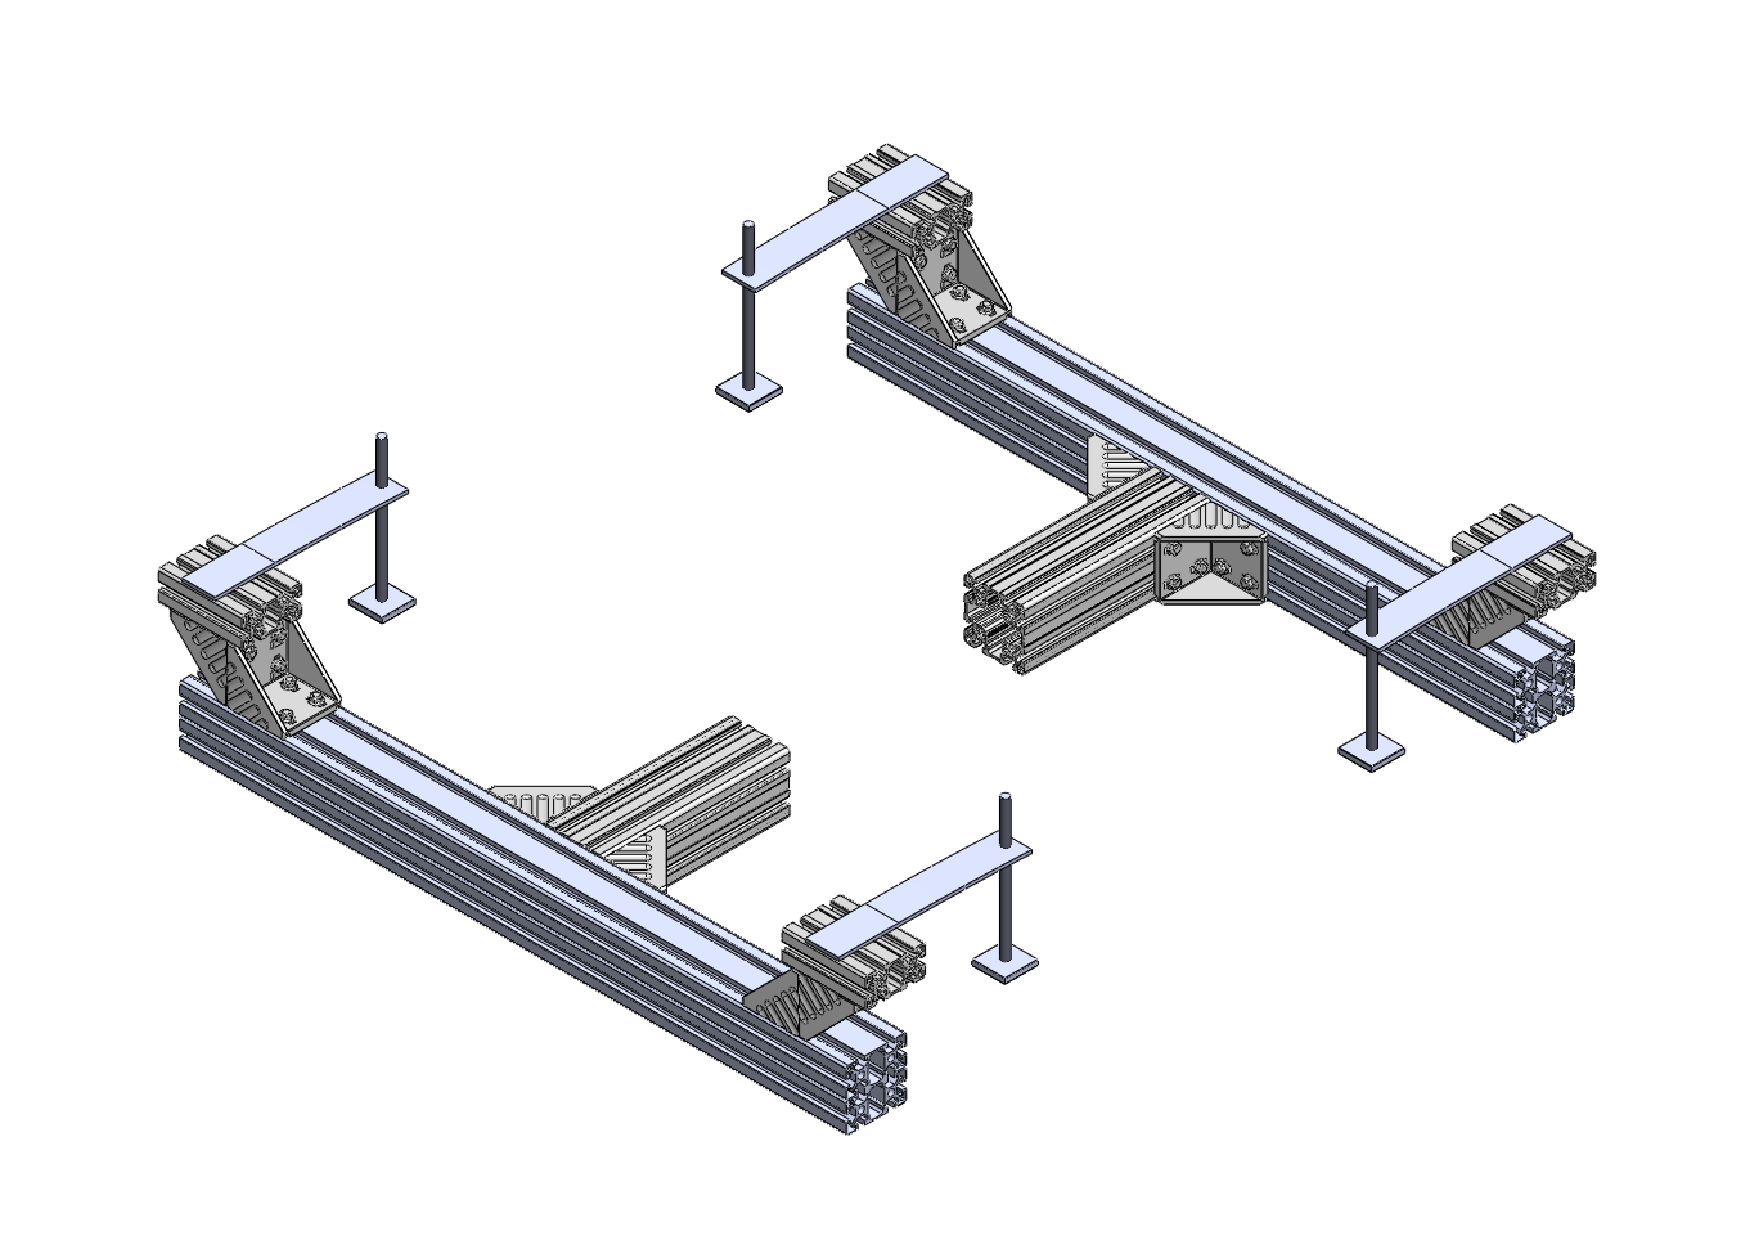
\includegraphics[width=0.80\textwidth]{Pictures/Waage_2Ansichten.pdf}
\caption{CAD-Modell des Wägesystems mit Blattfeder.}
\label{fig:}
\end{figure}

Während der Arbeit wurde ein Wägesystemkonzept entworfen und gebaut. Das Wägesystem hatte \textit{konstruktive} als auch \textit{messtechnische} Anforderungen zu erfüllen. Aufgrund wechselnder Verdampfer-Prüflinge und schneller Demontage des Prüflings inklusive Wägesystem aus der Klimakammer sollte das Wägesystem  kompakt, mobil, für mehrere Verdampferhalterungen variabel und demontierbar sein. 
Messtechnische Anforderungen an das Wägesystem waren:

\begin{itemize}
\item Ermittlung des gesamten Eisgewichtes am Verdampfer
\item Ermittlung des 2D-Schwerpunktes der Eismenge
\item Automatisiertes Datenauslesen mittels der SPS, beschrieben im Abschnitt \ref{sec:Informationstechnischer Aufbau}.
\end{itemize}

\subsection{Messtechnik}
\label{subsec:Waagen-Messtechnik}

Für das Wägesystem wurden 5 Waagen der Fa. \textsc{Kern und Sohn GmbH} verwendet. Die Waagen kommunizieren mit der SPS per RS-232 Schnittstelle. Das Kommunikationsprotokoll ist das 22-bit Protokoll, dass auf dem \textsc{ASCII}-7 bit- Zeichenkodierung beruht. \footnote{\textbf{ASCII} steht für \textit{American Standard Code for Information Interchange} und wurde im Jahre 1963  \textit{American Standards Association} gebiligt. Es war bis 2007 die meist verbreiteste 7-bit-Zeichenkodierung im World-Wide-Web, bis es von UTF-8 überholt wurde.}. Die Kommunikation zwischen der Waage und der SPS ist näher in \ref{sec:Informationstechnischer Aufbau} beschrieben und erläutert.

Das Wägeprinzip der eingesetzten Waagen beruht auf dem Dehnungsmessstreifen-Prinzip. Die Ablesegenauigkeit der Waagen korreliert mit dem max. Wägebereich. Der Waagentyp \textit{PCD 10K0.1} der Fa. Kern und Sohn GmbH ist ein guter Kompromiss aus Messbereich und -genauigkeit. Diese Waage kann  jeweils  bis 10 kg belastet  werden. Des Weiteren besitzt die Waage eine sehr genaue Ablesbarkeit. Da der Verdampfer auf vier Waagen stehen wird, die maximal mit 10 kg jeweils belastet werden können, muss die Konstuktion erstens die Eismenge gleichmäßig auf alle vier Waagen verteilen. Zweitens muss das Eigengewicht des Verdampfers mit der Konstruktion gehalten werden. 


 
\begin{table}[htb]
\centering
\caption{Waagendaten}\vspace{6pt}
\begin{tabular}{ll}
\hline 
 & \textbf{Waage}  \\ 
\hline 
\hline 
Typ & PCD 10K0.1 \\ 
\hline 
Hersteller & \textsc{Kern und Sohn Gmbh} \\ 
\hline 
Messbereich & 0..10 kg \\ 
\hline 
Ablesbarkeit & 100 mg\\ 
\hline 
max. Luftfeuchtigkeit & 80 $\%$\\
\hline
min. Umgebungstemperatur & 5 °C\\
\hline
max. Umgebungstemperatur & 35 °C\\
\hline
Kommunikationsart & RS-232 \\ 
\hline 
Hilfsenergie & 220-240  V   \\ 
\hline
Anzahl & 5 \\ 
\hline 
%Datenblatt(URL) &  \\ 
\hline 
\end{tabular} 
\label{tab:Waagendaten}
\end{table}



\subsection{Konstruktion}
\label{subsec:Waagen-Konstruktion}


Nach Entwicklungen von verschiedenen Konzepten und Prototypen wurde sich für ein Wäagesystem mit vier eingespannten Stahlblättern als Blattfedern entschieden.  Die Abbildung \ref{fig:Feder} zeigt die Federkonstruktion mit den auf die Feder wirkenden Kräften. Die Blattfeder ist mit einem Boschprofil verschraubt, dass die Lagerkräfte auf den Boden ableitet. Am Ende der Blattfeder ist eine 10 mm Gewindestange mit zwei Muttern befestigt. Durch diese Muttern lassen sich bei der späteren Kalibrierung die Vorspannung einstellen. Am oberen Ende der Gewindestange ist die Standgerüst des Verdampfers befestigt. Da es vier Aufhängungs- bzw. Lagerpunkte gibt, wird ca. $1/4$ der Gewichtskraft ($F_{Verdampfer}$) in jede Gewindestange eingeleitet. Am Fuß der Gewindestange ist eine 50 mm x 50 mm x 5 mm Eisenplatte mit einer zentrierten 10 mm Gewindebohrung befestigt. Über den Fuß findet die Gewichtsübertragung zwischen der Waage und dem restlichen System statt. Am Fuß selber wird zusätzlich ein 5 mm dicker Gummidämpfer angeklebt. Dieser beugt zum einen möglichen Verkratzungen und Eindellungen auf der Waagenoberfläche vor, zum anderen bewirkt der Gummidämpfer eine minimale Dämpfung des ganzen Systems. Die Konstruktion sieht vor, dass der Fuß im 90$°$-Winkel auf der Waage aufliegt. 

\begin{figure}
\centering		\includegraphics[page=7,width=1.10\textwidth]{Pictures/Feder.pdf}
\caption{Federkonstruktion nach dem Prinzip des einseitig eingespannten Balkens}
\label{fig:Feder}
\end{figure}






Die Federn sollen in Form einer Blattfeder gebaut sein, die über eine lineare Federkennlinie verfügt. Die Blattfedern sollen über der Länge $l$ verstellbar sein und nach dem Prinzip des einseitig eingespannten Balkens fungieren, vgl. Abschnitt \ref{sec:Federn}. 

 
\begin{table}[htb]
\centering
\caption{Feder-Daten}\vspace{6pt}
\begin{tabular}{ll}
\hline 
 & \textbf{Blattfeder}  \\ 
\hline 
\hline 
Werkstoff & Edelstahl\\
\hline 
Elastizitätsmodul E & 206 kN/mm$^2$ \\ 
\hline 
Höhe h x Breite b x Länge l & 5 mm x 50 mm x 185 mm\\
\hline
Verdampfergewicht $F_{Verdampfer}$/4 & 490,5 N\\
\hline
maximale Eismenge $F_{Eis}$/4 & 24,5 N\\
\hline
$F_{ges}$ & 515 N\\
\hline
\hline
\end{tabular} 
\label{tab:Federblattereigenschaften}
\end{table}

Die maximale Eismenge am Ende des Vereisungsvorgang wird zu 10 kg festgelegt. Der Verdampfer verfügt über ein Gesamtgewicht von 10 kg. Da 4 Waagen mit jeweils einer Blattfeder vorgesehen sind, werden für die Auslegung nur ein Viertel der gesamten Gewichtskraft berücksichtigt.  Die Gewichtskräfte ergeben sich zu:
\begin{equation*}
F_{Verdampfer}= 1/4\cdot 200 kg \cdot 9,81 m/s^2 = 490,5 N
\end{equation*}
\begin{equation*}
\Delta F_{Eis}= 1/4 \cdot 10 kg \cdot 9,81 m/s^2 = 24,5 N
\end{equation*}
\begin{equation*}
F_{ges}= F_{Verdampfer} + \Delta F_{Eis} = 515 N.
\end{equation*}

Die Federwege, nach Gleichung \ref{eq:Federweg}, je nach Belastung ergeben sich zu:

\begin{equation*}
  s(F= F_{Verdampfer})=9,65 mm 
 \end{equation*}
 \begin{equation*}
 s(F= F_{ges})= 10,13 mm 
 \end{equation*}
\begin{equation*}
 \Delta s(\Delta F_{Eis}) = 0,48 mm
\end{equation*}

Die Federrate $R$ ergibt sich zu:

\begin{equation*}
R = \frac{24,5 N}{1 mm} = 51,04 N/mm.
\end{equation*}

Die maximal auftretende Biegespannung ergibt sich bei $F_{ges}$ zu  $\sigma_{b,max} = 457,34 \frac{N}{mm^2}.$ Mit $R_m =1000 N/mm^2$, entnommen für Blattfedern aus TB 10-1 aus \citep{Wittel2011}, ergibt sich  $\sigma_{zul}\approx 0,7 \cdot 1100 N/mm^2 = 770 N/mm^2  $ als maximal zulässige Biegespannung. Daraus resultiert eine Sicherheit für die Blattfeder von:

\begin{equation}
S= \frac{770~N/mm^2}{457,34~N/mm^2} = 1,68.
\end{equation}





Diese Berechnung gelten für den Einsatz einer einzelnen Feder ohne Waage. Die Kombination aus einer Blattfeder und einer Waage hat Einfluss auf die Federrate und so auf den resultierenden Federweg des Wägesystems. Die Federrate wird größer, sprich die Feder wird härter. Aus einer härteren Feder resultiert ein kürzerer Federweg $\Delta s$.  In Abbildung \ref{fig:Feder_Waage_Fs} ist der verkürzte Federweg $\Delta s_{F+W}$ für ein System aus Feder und Waage dargestellt. Es folgt $\Delta s_{F+W}< \Delta s_{F}$. Die resultierende Federrate für eine Feder-Waage-Kombination ergibt sich aufgrund einer Parallelschaltung zu :

\begin{equation}
R_{F+W}= R_F + R_W.
\end{equation}

Die Federrate der Waage nicht bekannt. Eine gleichmäßige Verteilung des Verdampfersgewicht auf die vier Waagen könnte durch die Bestimmung der Durchbiegung aller Federblätter bestimmt werden. Eine praktische Auslesung des Federweges $s$ ist nicht vorhanden. Ungenaues Bestimmen würde zu großen Fehlern führen. Eine Abweichung von $\pm 0,1 mm$ zöge einen Messfehler von $\pm$ 0,5 kg nach sich.  Außerdem kann noch keine Aussage über den Schwerpunkt des gefrorenen Eises im Verdampfer getroffen werden.

\subsection{Kalibrierung}
\label{subsec:Waagen-Kalibrierung}


Erste Versuche mit dem Wägesystem führten zu der Erkenntnis, dass die Federn sich bei der Einstellung der Vorspannung sehr stark gegenseitig beeinflussen. 
 
Deshalb wird das Wägesystem und alle ihre Waagen vor jeder Messung kalibriert. Da ein Wägesystem aus Blattfedern einen bestimmten Teil des Gewichtes durch die Blattfedern ableiten und nur ein Bruchteil des belastenden Gewichtes an die Waagen weitergibt, gilt es diesen Teil zu bestimmen. Das Verhältnis von dem belastenden Gewichts bei der Waage ankommt wird im folgenden Umrechnungsfaktor $k$ genannt. Der Umrechnungsfaktor lautet formelmäßig:XY

\begin{equation}
tatsächliches ~Gewicht= \frac{angezeigtes~ Waagengewicht}{k}.
\label{eq:k}
\end{equation}

Das tatsächliche Gewicht, mit dem die Waage belastet wird, lässt sich zurückrechnen, wenn die Funktion von $k$ bekannt ist. 
Da das E-Modul der Blattfeder von der Temperatur abhängt, ist auch $k$ eine Funktion von der Temperatur. Da eine Belastung des Wägesystems auch eine Verschiebung des gesamten Schwerpunktes des Luftkühlers mit sich bringt, wird $k$ auch von der belastenden Masse abhängen. Folglich ist die Funktion des Umrechnungsfaktors gegeben durch: 

\begin{equation}
k_i = f_i(T,m). 
\end{equation}

Um die Funktion nur von der zu belastenden Masse abhängig zu machen, wird die Kalibrierung bei einer konstanten Temperatur in der Klimakammer durchgeführt. Bevor die Kalibrierung startet werden alle Waagen mit 2000 g vorgespannt und dann mittels des Offset-Programms auf Null gesetzt. Für das Offset-Programm ermittelt die SPS die aktuelle Belastung, mittelt diese über 60 Sekunden und subtrahiert diese dann von dem angezeigten Waagengewicht.
Für die Kalibrierung werden 5 Prüfgewichte (500...2500 g) zeitlich hintereinander genau über der Gewindestange platziert. Es folgt eine Einschwingphase des Wägesystems. Danach wird 60 Sekunden das angezeigte Waagengewicht aufgezeichnet und gemittelt. Da das genaue Gewicht der Prüfgewichte bekannt ist, kann $k$ für diesen Belastungspunkt errechnet werden. Nach Beendigung der Messphase ist das nächst höhere Gewicht an der Reihe. Dieser Vorgang wird durchgeführt bis alle vier Waagen mit allen Prüfgewichten belastet und gemessen worden ist. 
Der Umrechnungsfaktor kann nun für jede Waage und jede Belastungsmasse interpoliert bzw. extrapoliert werden.


Die gesamte Eismasse im Verdampfer ist die Summe aller angezeigten Gewichte geteilt durch den zugehörigen Umrechnungsfaktor:

\begin{equation}
m_{Eis}= \frac{m_1}{k_1}+ \frac{m_2}{k_2}+ \frac{m_3}{k_3}+\frac{m_4}{k_4}
\label{eq:Eismasse}
\end{equation}

Der Schwerpunkt(SP) wird berechnet aus den Anteilen der Waagen am gesamten Gewicht am Verdampfer multipliziert mit ihrer eigen Position. Der Nullpunkt des Koordinatenkreuzes wird auf die Mitte des Wärmeübertragers gelegt. Von hier wird dann der Ortpunkt jeder Waage ermittelt. Da nicht der ursprüngliche Schwerpunkt des gesamten Luftkühlers bekannt ist, kann durch die Schwerpunktsermittelung lediglich die Schwerpunktsverschiebung bestimmt werden. Diese Verschiebung wird auf den Mittelpunk des Wärmeübertrager referenziert und ist bei jedem Start der Messung gleich Null
Für die x-Koordinate der Schwerpunktsverschiebung gilt folgende Formel:
\begin{equation}
x_{SP} = \frac{x_1\cdot \frac{m_1}{k_1}+ x_2\cdot \frac{m_2}{k_2}+ x_3\cdot \frac{m_3}{k_3}+x_4\cdot \frac{m_4}{k_4}}{\frac{m_1}{k_1}+ \frac{m_2}{k_2}+ \frac{m_3}{k_3}+\frac{m_4}{k_4}}
\label{eq:SP}
\end{equation}

Hierbei ist $x_i$ die Position jeder Waage. Die y-Koordinate des Schwerpunktes wird analog zu Gleichung \ref{eg:SP} ermittelt. 

Die Ergebnisse der Kalibrierung sind im Abschnitt \ref{sec:Waegesystem} nachzulesen.  
Der Kalibrierungsprozess wird in die Software implementiert, siehe Abschnitt \ref{sec:Informationstechnischer Aufbau} für den informationstechnischen Aufbau. 






%\begin{figure}[htb]
%\centering		\includegraphics[width=0.90\textwidth]{Pictures/%Feder_Waage_Fs.pdf}
%\caption{Kraft-Weg-Kennlinie mit Federweg für System aus Feder(F) %und System aus Feder und Waage (F+W)}
%\label{fig:Feder_Waage_Fs}
%\end{figure}

